\documentclass{beamer}
\usetheme{metropolis}

\usepackage{array}
\usepackage{caption}
\usepackage{graphicx}
\usepackage{xcolor}

\title{Communication in Multi-agent Reinforcement Learning}
\date{\today}
\author{Jack Montgomery}
\institute{MAM4001W: Advanced Topics in Reinforcement Learning}

\begin{document}

\maketitle

\section{Motivation}
\begin{frame}{Motivation}
\begin{figure}
	\centering
	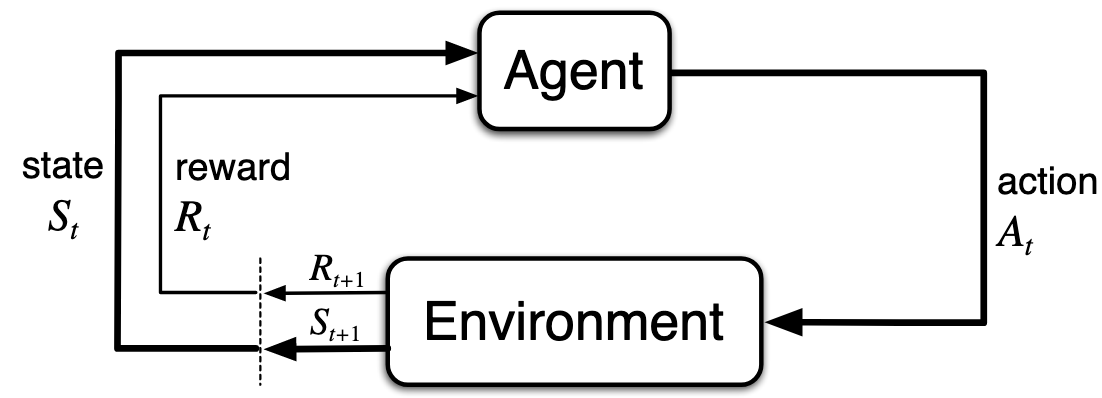
\includegraphics[scale=0.4]{images/agent_environment.png}
\end{figure}
\end{frame}

\begin{frame}{Motivation}
\begin{figure}
	\centering
	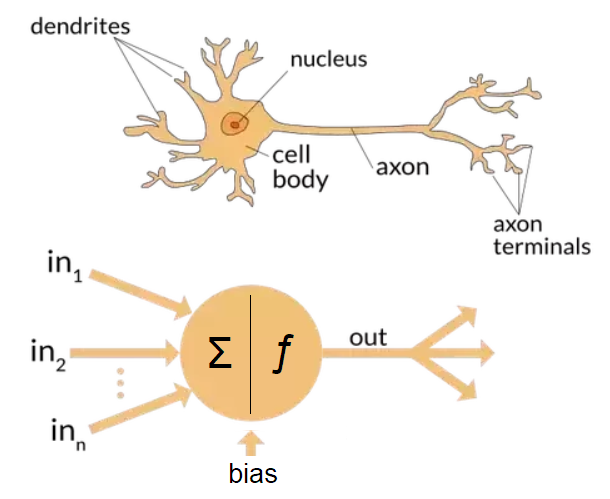
\includegraphics[scale=0.4]{images/neural_networks.png}
\end{figure}
\end{frame}

\begin{frame}{Motivation}
\begin{itemize}
	\item Non-stationarity
	\item Credit Assignment
	\item Scaling
\end{itemize}
\end{frame}


\section{Comm-MARL}
\begin{frame}{How do we communicate?}
	\begin{figure}
		\centering
		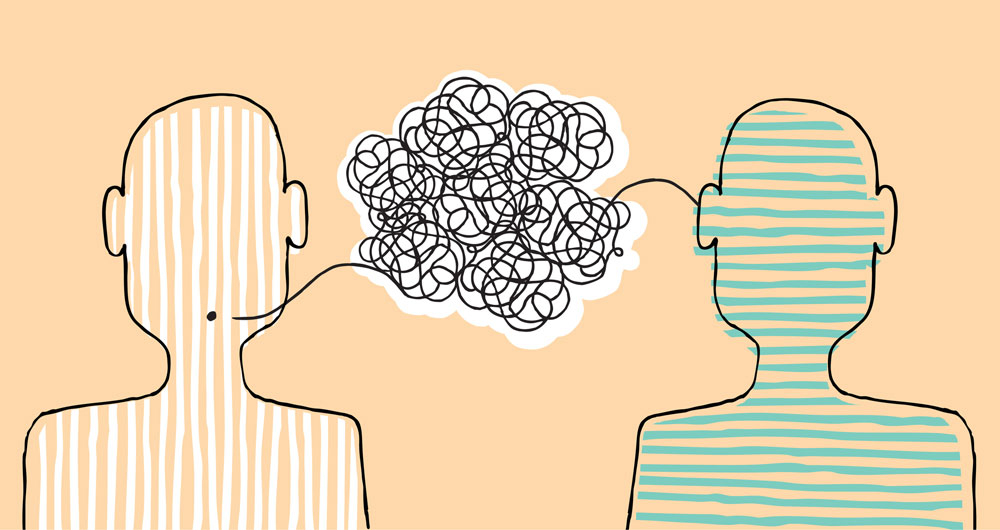
\includegraphics[scale=0.3]{images/communicate.jpg}
	\end{figure}
\end{frame}

\begin{frame}{Dimensions of Comm-MARL}
    \scriptsize 
    \resizebox{\textwidth}{!}{
        \begin{tabular}{|>{\centering\arraybackslash}m{2.8cm}|>{\centering\arraybackslash}m{1cm}|>{\arraybackslash}m{5.5cm}|>{\centering\arraybackslash}m{2.8cm}|}
            \hline
            \textbf{Component} & \textbf{Index} & \textbf{Question} & \textbf{Dimension} \\
            \hline
            Problem Setting
            & 1 & What kind of behaviours are desired to emerge with communication? & Controlled Goals \\
            \cline{2-4}
            & 2 & How to fulfil realistic requirements? & Communication Constraints \\
            \cline{2-4}
            & 3 & Which type of agents to communicate with? & Communicatee Types \\
            \hline
            Communication Processes
            & 4 & When and how to build communication links among agents? & Communication policy \\
            \cline{2-4}
            & 5 & How to combine received messages? & Message combination \\
            \cline{2-4}
            & 6 & Which piece of information to share? & Communicated messages \\
            \cline{2-4}
            & 7 & How to integrate combined messages into learning models? & Inner integration \\
            \hline
            Training Processes 
            & 8 & How to train and improve communication? & Learning methods \\
            \cline{2-4}
            & 9 & How to utilise collected experience from agents? & Training schemes \\
            \hline
        \end{tabular}
    }
\end{frame}

\begin{frame}{Dimensions of Comm-MARL}
    \scriptsize 
    \resizebox{\textwidth}{!}{
        \begin{tabular}{|>{\centering\arraybackslash}m{2.8cm}|>{\centering\arraybackslash}m{1cm}|>{\arraybackslash}m{5.5cm}|>{\centering\arraybackslash}m{2.8cm}|}
            \hline
            \textbf{Component} & \textbf{Index} & \textbf{Question} & \textbf{Dimension} \\
            \hline
            Problem Setting
            & 1 & What kind of behaviours are desired to emerge with communication? & Controlled Goals \\
            \cline{2-4}
            & 2 & How to fulfil realistic requirements? & Communication Constraints \\
            \cline{2-4}
            & 3 & Which type of agents to communicate with? & \textcolor{red}{Communicatee Types} \\
            \hline
            Communication Processes
            & 4 & When and how to build communication links among agents? & Communication policy \\
            \cline{2-4}
            & 5 & How to combine received messages? & Message combination \\
            \cline{2-4}
            & 6 & Which piece of information to share? & \textcolor{red}{Communicated messages} \\
            \cline{2-4}
            & 7 & How to integrate combined messages into learning models? & Inner integration \\
            \hline
            Training Processes 
            & 8 & How to train and improve communication? & \textcolor{red}{Learning methods} \\
            \cline{2-4}
            & 9 & How to utilise collected experience from agents? & Training schemes \\
            \hline
        \end{tabular}
    }
\end{frame}

\begin{frame}{Method}
	\begin{enumerate}
		\item RIAL and DIAL
		\item CommNet
		\item IC3Net
		\item BiCNet
		\item NeurComm
		\item HAMMER
	\end{enumerate}
\end{frame}

\begin{frame}{Commuicateee Types}
\begin{itemize}
	\item Nearby Agents
	\item Other Learning Agents
	\item Proxy
\end{itemize}
\end{frame}

\begin{frame}{Communicated messages}
\begin{itemize}
	\item Existing knowledge
	\item Imagined future knowledge
\end{itemize}
\end{frame}

\begin{frame}{Learning Methods}
\begin{itemize}
	\item Reinforced
	\item Differentiable
\end{itemize}
\end{frame}

\section{Parameter Sharing}

\begin{frame}{NPS vs PS Model}
	\begin{figure}
		\centering
		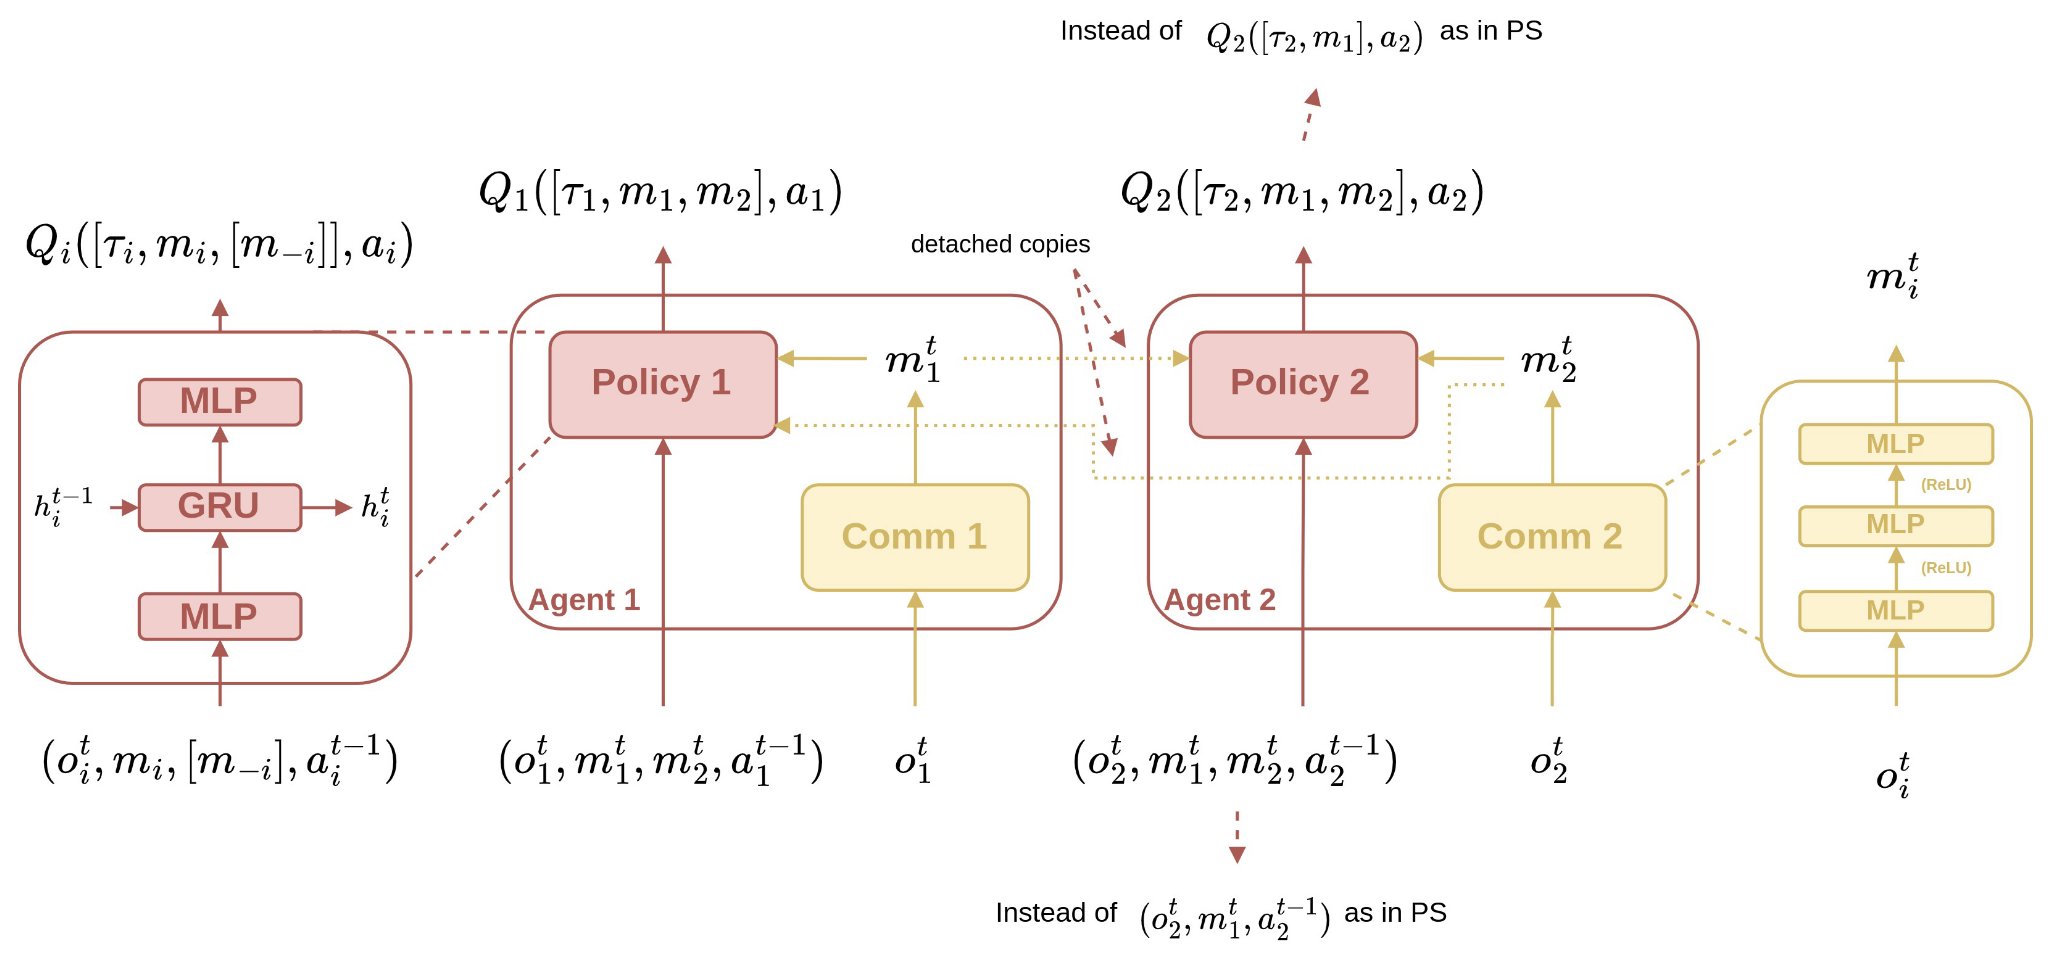
\includegraphics[scale=0.25]{images/nps_comm.png}
	\end{figure}
\end{frame}

\begin{frame}{Results}
	
\end{frame}

\end{document}